
\documentclass{article}
\usepackage{amsmath} 
\usepackage{blindtext}
\usepackage[a4paper, total={6in,6in}]{geometry}
\usepackage{graphicx}
\begin{document}
\section{Introduction}
% \includegraphics[scale=0.2]{../gsplines.svg}
$f(\phi(u,v))=g(u,v)$

\begin{equation}
\label{eqn:G1}\phi(x,0)=(x,0)
\end{equation}

$\phi=(\phi_1,\phi_2)$

implies the folowing:

$y \,  divides \,\phi_2(x,y)$

ie

$\phi_2(x,y)=y.k(x,y)$

and:

$\phi_1(x,y)=x +y.q(x,y)$

for some polynomials $q,k$.

\section{Gk conditions}
the Gk are all the partial derivative of order less than k of $f(phi) $ and $g$ are equale.


\section{G1 Equation}

Because of the \ref{eqn:G1} the jacobian of $\phi$ is of the forme:

$$D\phi=
\begin{pmatrix}
1&a(u,v)\\
0 &b(u,v)
\end{pmatrix}
$$
a and b are functions of u,v.

and the G1 condition: $\partial _v g=a(u,v)\, \partial _u f (\phi)+b(u,v)\, \partial _v f (\phi)$  with $v=0$.
can also be written:
$$\partial _v g=(\partial _u f (\phi),\partial _v f (\phi)) \begin{pmatrix} a\\b\end{pmatrix}$$

\section{G2 condition}

$$\partial ^2_vg=(a,b)(DDf)(\phi)\begin{pmatrix} a\\b\end{pmatrix}+Df(\phi) \partial_v\begin{pmatrix} a\\b\end{pmatrix}$$
$DDf $ is the hessian of $f$.
\end{document}
